\documentclass[../manuale_sviluppatore.tex]{subfiles}

\begin{document}

\subsection{Pattern architetturale: }

\subsection{Architettura di dettaglio}

\begin{figure}[H]
	\centering
	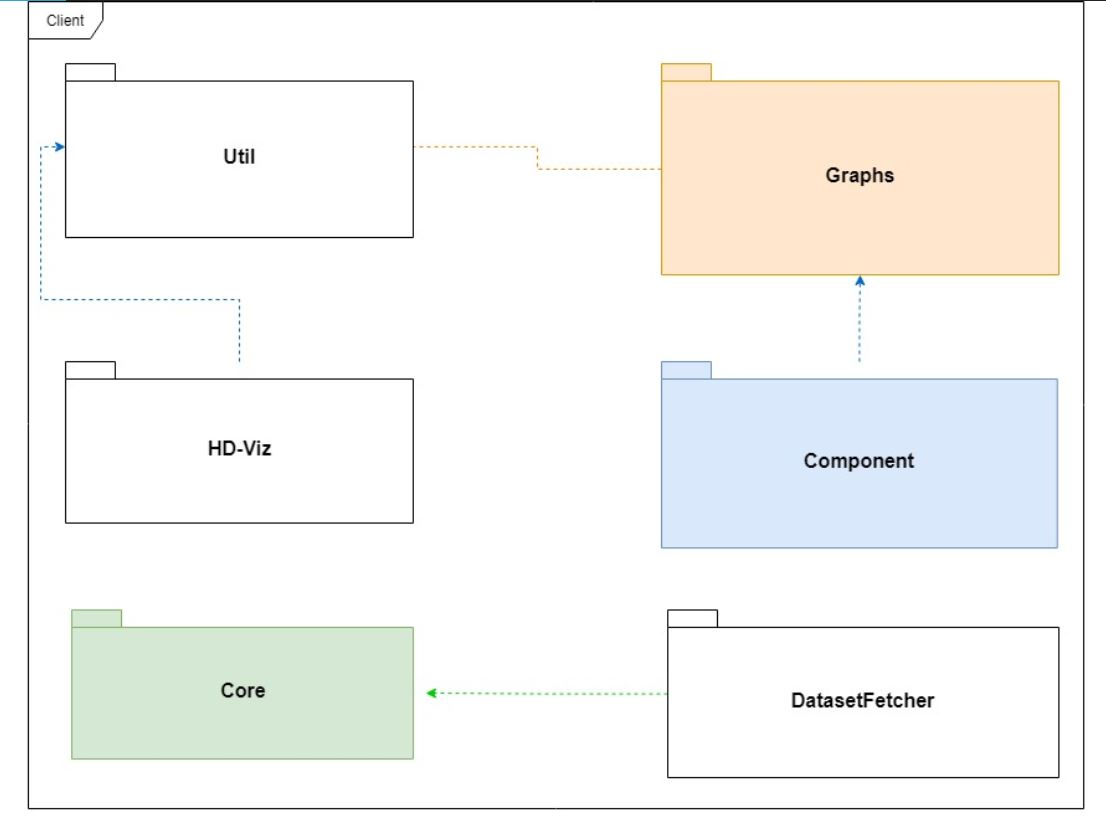
\includegraphics[width=18cm]{img/core.jpg}
	\caption{Introduzione a Hd-Viz}
\end{figure}

\emph{HD Viz manager} è il core dell'architettura, si delegherà la visualizzazione ai vari Manager, inoltre terrà traccia 
dei dati per evitare istanze multiple del Dataset, della DistanceMap e dei grafici una volta creati. Nel momento in cui 
verrà modificato il dataset per modificare le visualizzazioni, farà da tramite creando una copia del dataset originale e usando
tali copie per le modifiche, cosicchè il dataset originale resti invariato.
Collaborerà poi assieme al \emph{GraphCreatorManager} che gestirà le factories per i vari modelli dei grafici. 
Il \emph{CurrentGraphManager} verificherà se le factories saranno in grado di costruire il grafico, quindi comunicherà con il 
presenter e il modello del grafico relativo. \\


\begin{figure}[H]
	\centering
	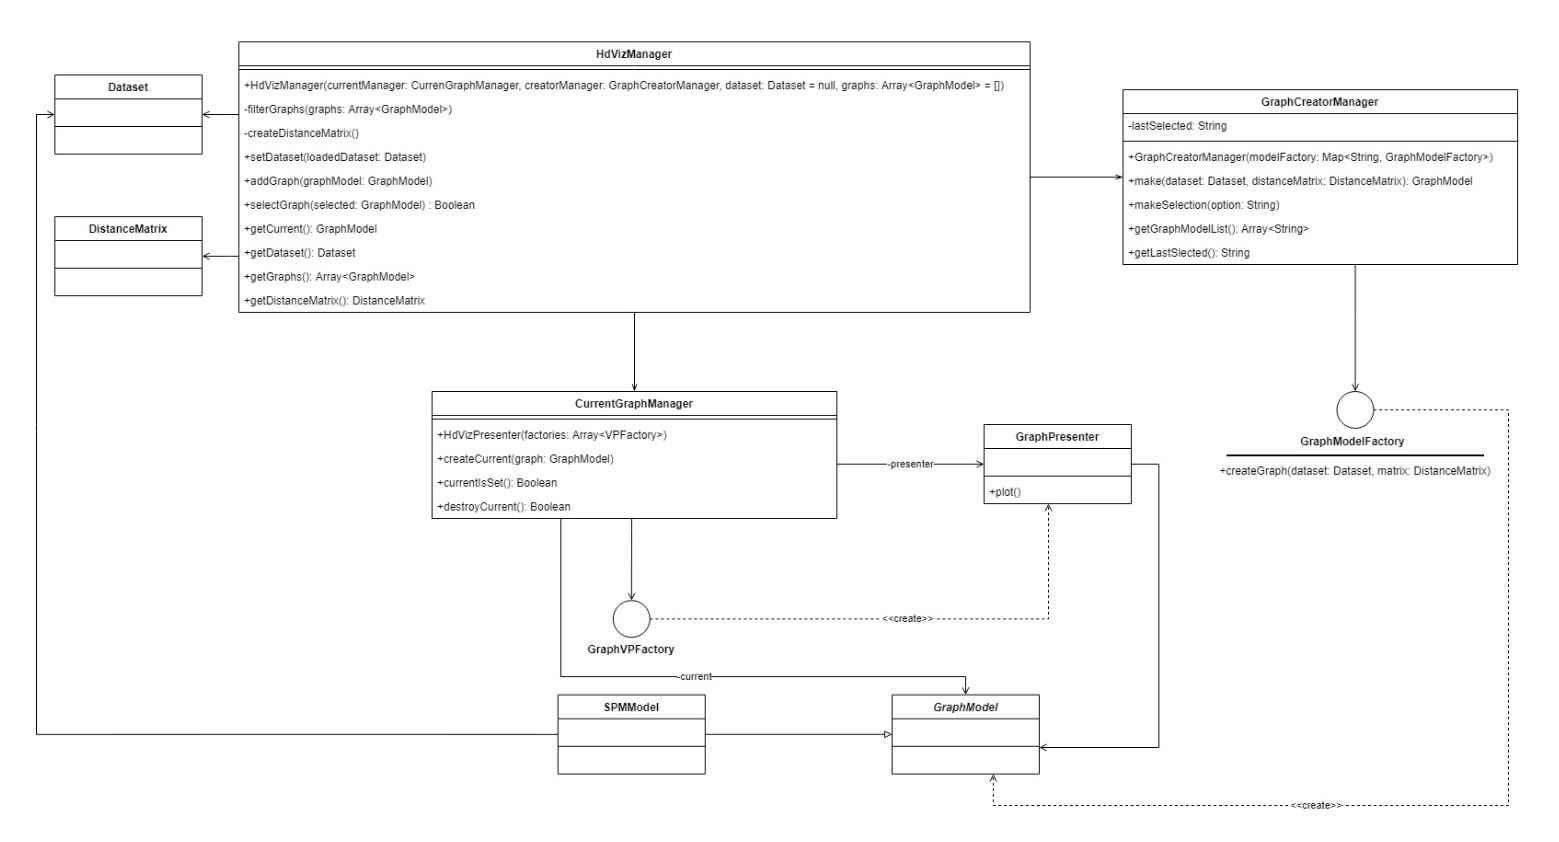
\includegraphics[width=18cm]{img/core-hdvizmanager.jpg}
	\caption{Introduzione a Hd-Viz}
\end{figure}

Graphs contiene le diverse visualizzazioni che la nostra applicazione metterà a disposizione, Component mette a disposizione una serie di componenti che permettono di aggiungere funzionalità ai grafici.
Questi ultimi modificano le proprietà di visualizzazione dei grafici, dialogando con modelli tramite interfacce. Ciascun component ha un \emph{Presenter} che gestisce la logica e la \emph{View} che renderizza il tutto,
infatti tramite le interfacce ogni grafico implementerà dimensioni e colori a modo proprio.

\begin{figure}[H]
	\centering
	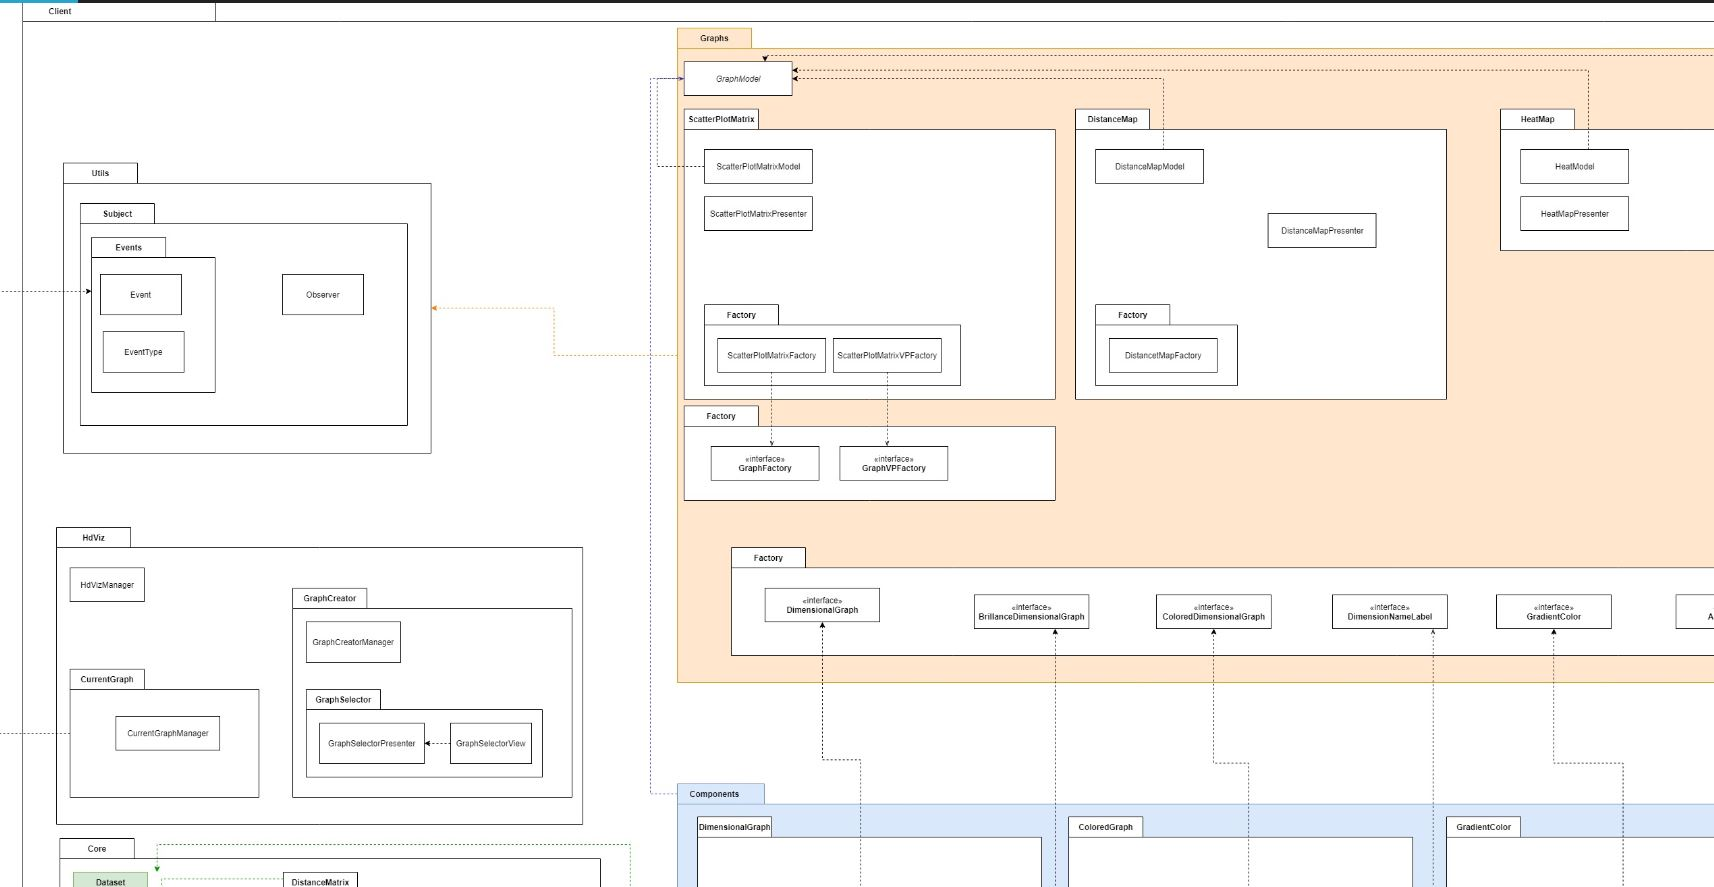
\includegraphics[width=18cm]{img/graph-e-hdviz.jpg}
	\caption{Introduzione a Hd-Viz}
\end{figure}


Ciascun grafico eredita il \emph{GraphModel}; dentro il modello salverà le impostazioni del grafico, ad esempio il gradiente colori, il dataset, i label delle righe ecc.

\begin{figure}[H]
	\centering
	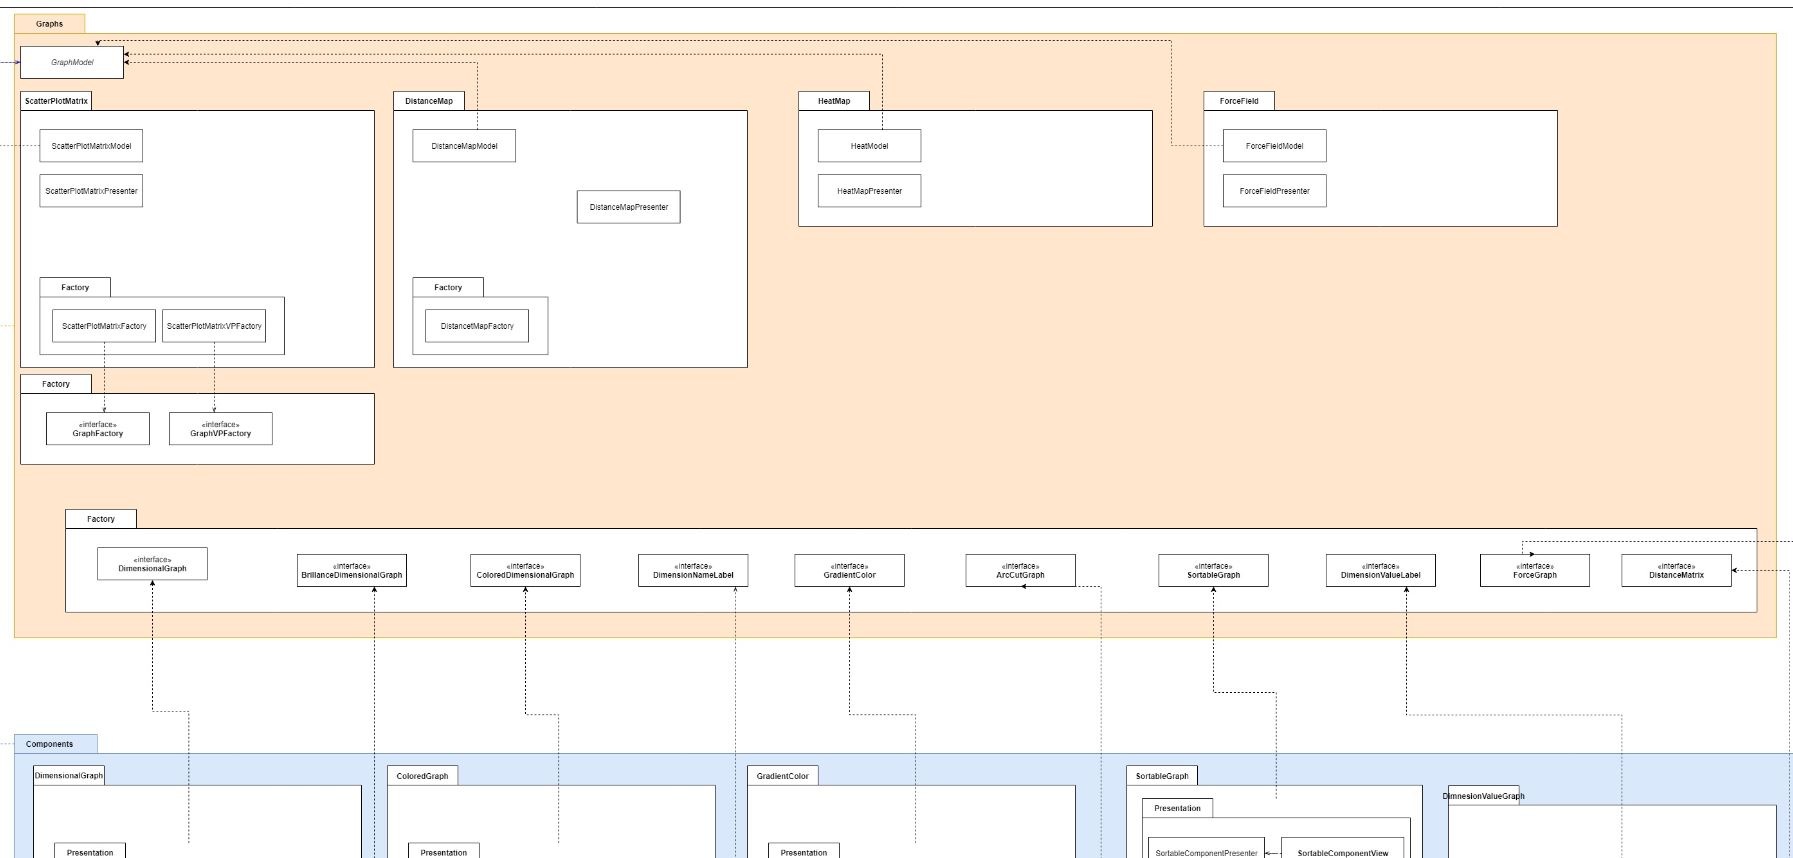
\includegraphics[width=18cm]{img/graphs-e-components.jpg}
	\caption{Introduzione a Hd-Viz}
\end{figure}


Collegando il model al presenter, i vari componenti che modificano la visualizzazione notificheranno il model, che si aggiornerà, e dirà al presenter di aggiornarsi perchè la visualizzazione è cambiata. 
Ciò avverrà tramite i metodi update. In particolare verrà aggiornato l'EventType.

\end{document}